Age of Swag : Conquest CMI est un jeu amateur libre et gratuit conçu par des étudiants à l'Université de Cergy-Pontoise, développé en Java à l'aide de la librairie graphique LibGdx.\\

Avant de vous lancer dans l'aventure de Age of Swag, nous vous recommandons de lire ce mode d'emploie pour savoir comment jouer mais aussi connaître les conseils indispensables.\\

Age of Swag vous propose un support technique gratuit et hors pair, disponible 24/24h 7/7j aux adresses mails suivantes :\\
  \begin{itemize}
    \item bastien-12@hotmail.fr
    \item lucas.nicosia@yahoo.fr
    \item aryus96@hotmail.fr
  \end{itemize}
    
    Attention, cette assistance s'adresse seulement aux bénéficiaires de notre projet Age Of Swag.\\

\section{Configuration requise}
Age of Swag : Conquest CMI fonctionne sur divers systèmes
tels que Windows, Linux ou Mac OS X. Etant libre, elle peut être facilement
portée sur d'autres systèmes (contactez-nous).
Nous avons fait de notre mieux pour optimiser la programmation, mais le
jeu utilise tout de même un minimum de ressources, donc il risque de ne
pas être jouable correctement sur des ordinateurs relativement peu
puisssants.
Les performances diffèrent selon les machines et il est difficile d'établir
précisément une configuration minimale. Nous vous conseillons quoi qu'il
en soit de fermer toutes les autres applications actives quand vous jouez à
Age Of Swag : Conquest CMI.\\

Age Of Swag à été testé sur divers configuration, et à été jugé parfaitement fonctionnel par notre équipe sur ces configurations :\\
  \begin{itemize}
    \item i7-3630QM (2.4Ghz)- Nvidia GT740M - 16Go de RAM
    \item i5-3230M (2.6GHz) - Nvidia NVS 5200M - 8Go de RAM
    \item i5 650 (3.20Ghz )- AMD Radeon HD 5700 Series - 4Go de RAM\\
  \end{itemize}
  \section{Configuration le jeu}
  \textbf{Installer Age of Swag : Conquest CMI}\\
  
  Pour installer et démarrer Age Of Swag, rien de plus simple, il suffit d'installer la dernière Java Runtime Environment (Pour plus d'informations sur l'obtention de la derniere Java Runtime Environment, connectez-vous à l'adresse suivante \url{http://www.oracle.com/technetwork/java/javase/downloads/jre8-downloads-2133155.html}.

  Si vous disposez déjà de Java Runtime Environment ou que vous venez de l'installer, il vous suffit juste de double cliquer sur l'exécutable .jar du projet.\\
  
    \textbf{Désinstaller Age of Swag : Conquest CMI}\\
    
    Il vous suffit de supprimer l'exécutable .jar .\\
    
    \section{Jouer à Age of Swag : Conquest CMI}
	     
    \underline{Modes de jeu}\\ 
     
 \begin{enumerate}
\item Normal
 Dans ce mode, la carte est généré aléatoirement mais vous pouvez choisir le nombre de joueurs humain, le nombre de joueurs géré par l'ordinateur et si vous voulez qu'ils soient agressifs ou défensifs.\\
\item Aléatoire.\\
 Dans ce mode, la carte est généré aléatoirement, vous pouvez choisir le nombre de joueurs humain, ainsi que ceux gérés par l'ordinateur mais vous ne pouvez pas choisir leurs stratégies de combats.\\
\end{enumerate}     
     
     \underline{Local}\\
     
     \begin{enumerate}
\item Démarrez le jeu.
\item Appuyez sur le 1er bouton, New Game/Nouvelle partie.
\item Appuyez sur Local.
\item Dès lors, choisissez votre mode de jeux.\\
\end{enumerate}
     
     \underline{En ligne}\\
         \begin{enumerate}
\item Démarrez le jeu.
\item Appuyez sur le 1er bouton, New Game/Nouvelle partie.
\item Appuyez sur Online.
\item Choisissez si vous créez la partie ou rejoignez une partie.\\
\end{enumerate}
    
     \underline{Charger une partie}\\
         \begin{enumerate}
\item Démarrez le jeu.
\item Appuyez sur le 2nd bouton,Load game/Charger une partie.
\item Sélectionnez votre partie précédemment enregistré.
\end{enumerate}


     \underline{Editeur}\\
         \begin{enumerate}
\item Démarrez le jeu.
\item Appuyez sur le 3ème bouton,Load game/Charger une partie.
\item Créer votre carte avec le nombre de joueurs voulu.\\
\end{enumerate}


\section{Autres informations}

 \underline{Remporter la partie}\\
Pour gagner la partie, vous devrez conquérir l'intégralité des capitales ennemis à l'aide de vos troupes.\\
 
 \underline{Former une unité}\\
Afin de former une unité vous devez sélectionner votre capitale ou bien un territoire possédant une caserne. Vérifiez que vous avez bien les ressources nécessaire à sa formation, puis patienter le nombre de tours exigé pour l'unité. Attention, les casernes et capitales ne peuvent former que une unité à la fois.\\
  
   \underline{Créer un bâtiment}\\
Afin de créer un bâtiment, vous devez sélectionner un territoire autre que votre capital, vous appartenant et appuyer sur le bouton de création du bâtiment souhaité, attention, vérifier bien d'avoir les ressources nécessaires, puis vous devrez patienté un certains nombre de tour. \\
 
 \underline{Taille de la carte}
 La taille de la carte dans le mode éditeur est fixe.
 La taille dans les autres modes dépends du nombre de joueurs que vous mettez dans la partie.\\
 \\
 \underline{Types de territoires}\\
 \\
 Il existe 5 types de territoires : \\
 \begin{itemize}
    \item Forestier\\
    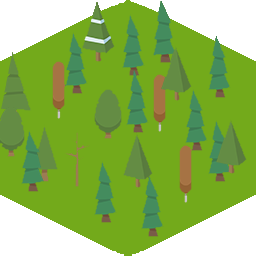
\includegraphics[scale=0.31]{ground/fo.png}\\
    \item Montagneux\\
    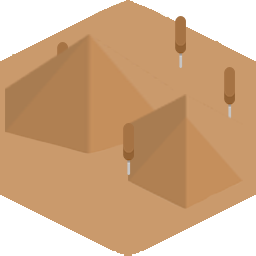
\includegraphics[scale=0.31]{ground/mo.png}\\
    \item Désertique\\
    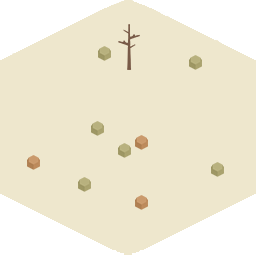
\includegraphics[scale=0.31]{ground/de.png}\\
    \item Aquatique\\
    
\includegraphics[scale=0.31]{ground/wa.png}\\
    \item Plaine\\
    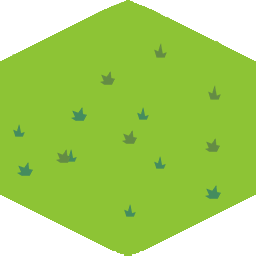
\includegraphics[scale=0.31]{ground/pl.png}\\
  \end{itemize}
    Les territoires Désertique et aquatiques sont les seuls qui vous seront infranchissable.\\
  \\
  \underline{Types de troupes}\\
  Age of Swag dispose actuellement de 5 types de troupes :\\
   \begin{itemize}
    \item    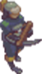
\includegraphics[scale=0.31]{troops/bow.png} Archer\\
   L'archer sera intéressant par son faible coût, temps de production et son attaque.\\
    ATK : 15\\
    DEF : 10\\
    2 tours de constructions et un coût de 20 ressources.\\
    
    \item 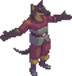
\includegraphics[scale=0.31]{troops/wiz.png} Magicien\\
     Le magicien possède la plus grande puissance d'attaque mais son coût et temps de production font de lui une arme stratégique.\\
    ATK : 25\\
    DEF : 5\\
    3 tours de constructions et un coût de 30 ressources.\\
    
    \item 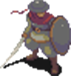
\includegraphics[scale=0.31]{troops/sword.png}  Épéiste\\
         L'épéiste tient sa force dans sa neutralité, l'équilibre de ces caractéristiques font de lui un soldat de choix.\\
    ATK : 15\\
    DEF : 15\\
    2 tours de constructions et un coût de 25 ressources.\\
    
    \item 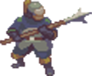
\includegraphics[scale=0.31]{troops/spear.png}  Lancier\\
             Le Lancier est une troupe de choix dans le cas d'une défense de territoire.\\
    ATK : 10\\
    DEF : 20\\
    2 tours de constructions et un coût de 25 ressources.\\
    \item 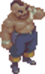
\includegraphics[scale=0.31]{troops/barbare.png}  Barbare\\
                 Le barbare est le soldat le plus basique du jeux. Il est néanmoins intéressant par sa rapidité de production et son faible coût.\\
    ATK : 10\\
    DEF : 10\\
    1 tours de constructions et un coût de 20 ressources.\\
  \end{itemize}

  \underline{Types de bâtiments}\\
  Age Of Swag : Conquest CMI dispose également de 3 types de bâtiments. \\
     \begin{itemize}
    \item l'Usine\\
    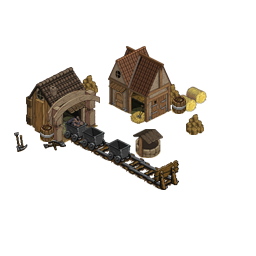
\includegraphics[scale=0.3]{bat/fac.png}\\
  L'usine va permettre d'augmenter la production des ressources sur le territoire sur lesquels vous l'avez construits, attention toutefois, chaque territoires possèdent un stock de ressources, il est judicieux de placer des usines à certains endroits.\\
    
    \item Caserne\\
    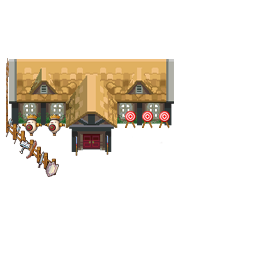
\includegraphics[scale=0.3]{bat/bar.png}\\
     La caserne vous permettras de créer des troupes hors de la capitale mais aussi de produire d'avantage de troupes par tours.\\
    
    \item Défense\\
    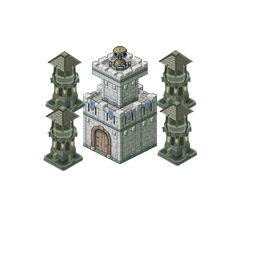
\includegraphics[scale=0.3]{bat/ram.png}\\
         Le bâtiment de défense va permettre à vos troupes de gagner en défense et donc de mieux résister aux assauts des troupes ennemis.\\
    
  \end{itemize}
   \textbf{Interface }\\
 \\
  \begin{center}
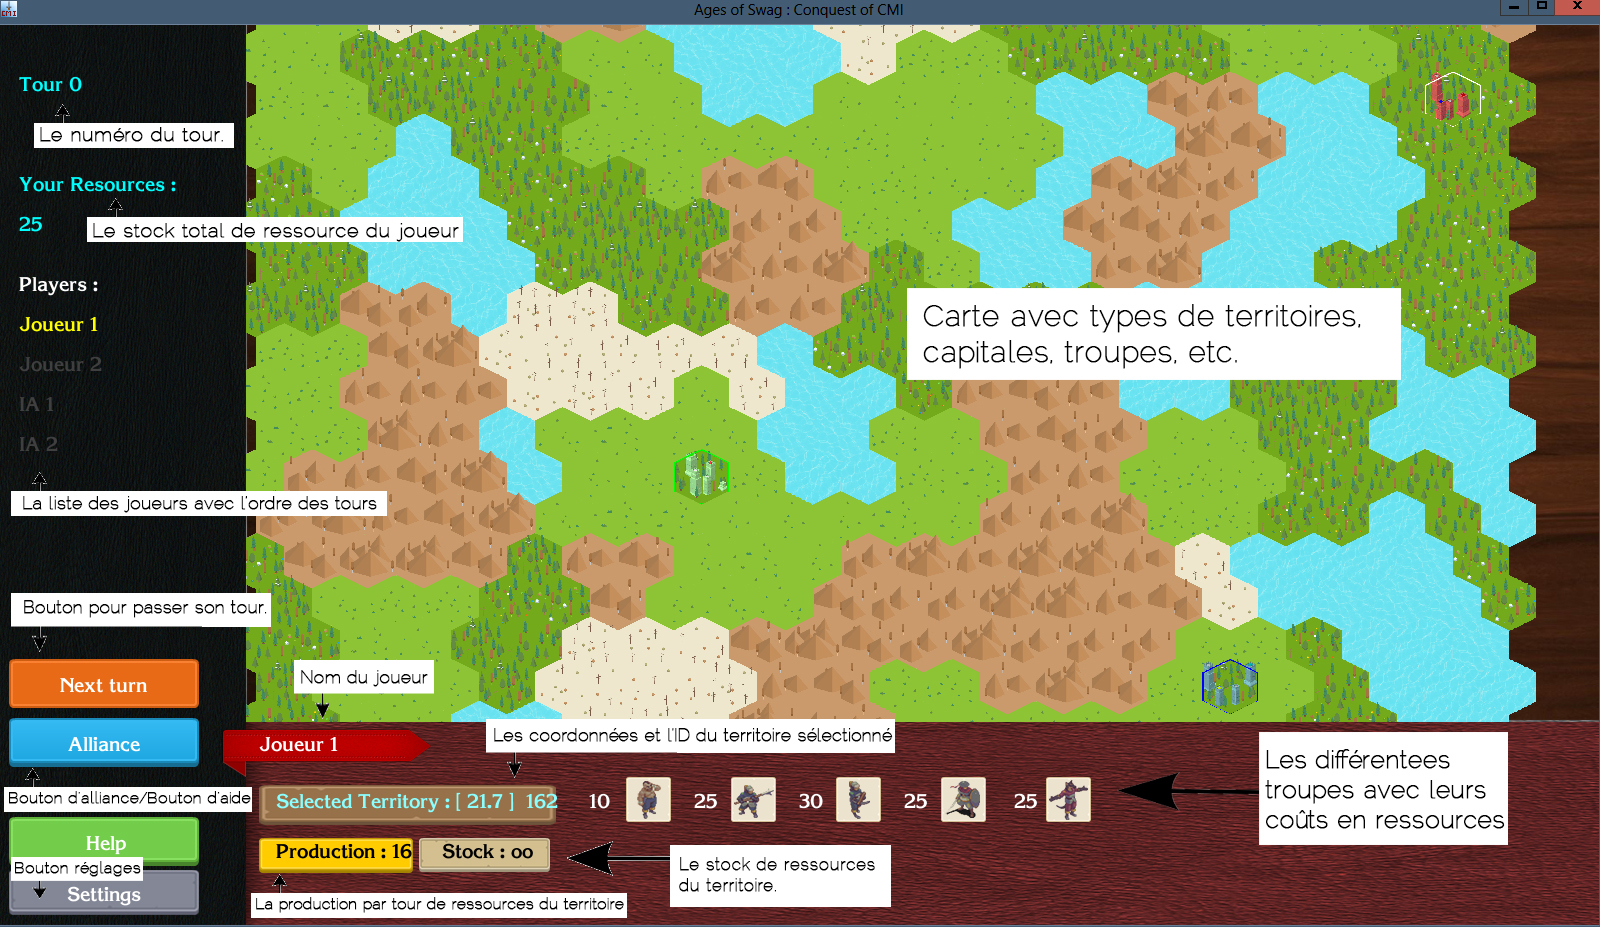
\includegraphics[scale=0.31]{help.jpg} \\
\end{center}

   \textbf{Modifier les options de jeu}\\

Les options de Age Of Swag sont relativement basique, vous avez la possibilité de changer la langue du jeu mais aussi de désactiver le son (seulement à partir du menu principal).\\
   
   \textbf{Pour afficher l'aide}\\
   Si vous souhaitez avoir de l'aide et des informations lors du jeux, vous pouvez cliquer sur le bouton vert aide/help qui vous donneras un panel d'informations sur le fonctionnement du jeu.